\chapter{EARLY INVESTIGATION: PROCESSING INSTRUCTIONS}
\label{insn}
After analyzing and experimenting with the hardware abstraction problems in
network switch devices, the focus shifted to the other end of the spectrum:
translating high level instructions. Not every hardware component in a system
needs to be abstracted up to the user level, but they need to be properly
utilized. In this chapter, two approaches to solving the translation problem
are considered. The first uses the extensible ISA named RISC-V in Section
\ref{insn:riscv}, and the second evaluates the usage of the HSA intermediate
representation, HSAIL \cite{hsail}, in Section \ref{insn:hsail}. In Section
\ref{insn:native}, the conclusions from each path of processing instructions
from high level languages are evaluated.

\section{RISC-V}
\label{insn:riscv}
RISC-V provides a base ISA that leaves room for the addition of custom, user
defined instructions that can be executed natively on a CPU architecture that
implements the ISA. For a network switch VM, this ISA is well suited to be a
natively supported ISA, as common network application instructions can be
optimized.

\begin{figure}[h!]
  \centering
  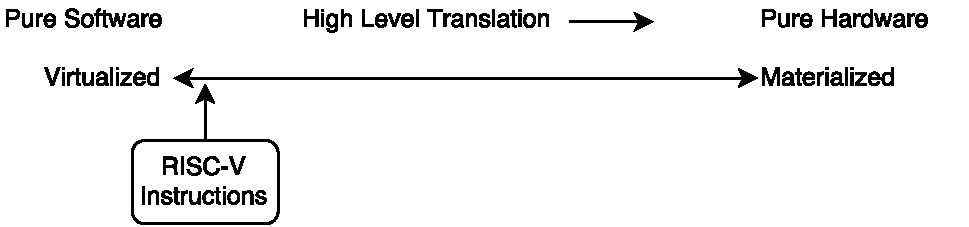
\includegraphics[scale=0.75]{spectrum_riscv}
  \caption{RISC-V currently relies on virtual CPU's that natively execute the
  ISA. Without a physical device, the instructions must be interpreted.}
  \label{spectrum_riscv}
\end{figure}

\section{HSAIL}
\label{insn:hsail}
\cite{hsail}

\section{Native Machine Code}
\label{insn:native}
To execute native code what resources do you need to provide?
